\section{Comparison of modern Java Script Frameworks}

\subsection{Overview}

There is a huge and steadily increasing amount of new JavaScript MVC frameworks.
A good overview over existing projects is provided by the Todo MVC App \enquote{tech-ana:todo-mvc}.
The Todo MVC app was created with the intention to help developers selecting a JavaScript framework by providing implementations of the very simple and ever same ToDo App, which allows to define a set of tasks that can be marked as done or undone.

%The application allows to add/delete/edit todo tasks and to mark/unmark tasks as done/undone.

The TodoMVC app gives also a good evidence of the rapid increase of existing JavaScript MVC frameworks.
Figure \ref{fig:todoMvcComp} shows a screenshot of the ToDoMVC taken at two different dates within a period of more than a year.

\begin{figure}
	\centering	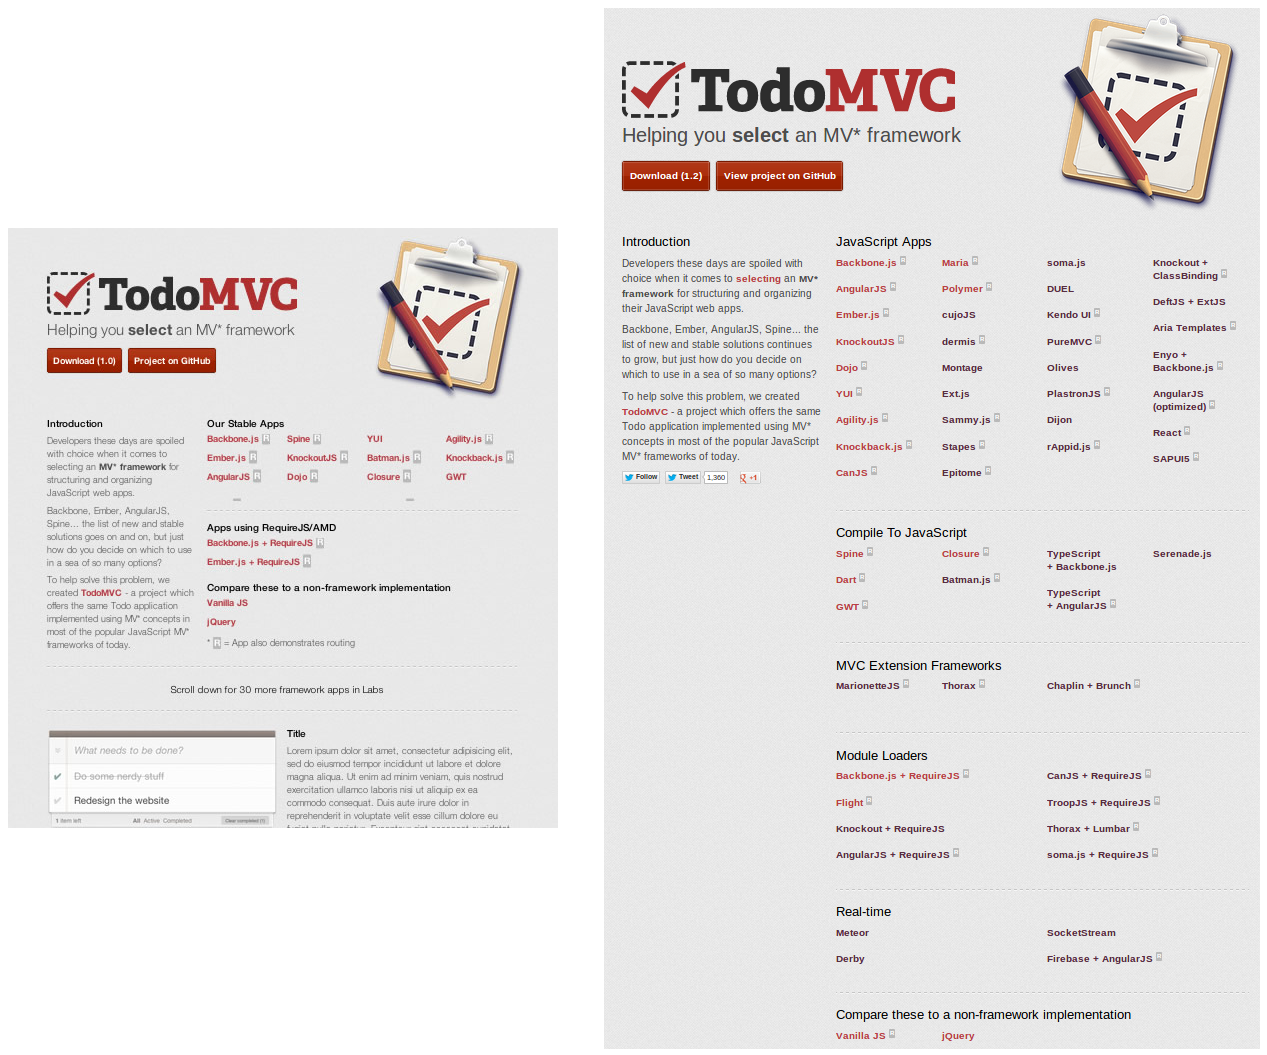
\includegraphics[width=1.0\textwidth]{./img/tech-ana/todo_mvc_app_comparison.png}
	\caption{Screenshot TodoMVC app left:July 2012, right: December 2013}
	\label{fig:todoMvcComp}
\end{figure}

The large amount of different frameworks makes it impossible to examine them all in detail.
Therefore a two step approach to filter the best suiting candidate is applied.
In a first step a very rough comparison of the frameworks is made to filter out the most inappropriate frameworks.
The remaining frameworks are then examined in more detail in chapter \ref{chap:detail_comparison}.
Furthermore a simple application is implemented with each framework that is selected for the detailed comparison to get a better understanding of the concepts used there.
The implemented application is a Simple Greeting Application where a user can edit its first and last name and then sees a greeting. 
It is obvious that the complexity of this demo application is not sufficient to demonstrate all strenghts of the frameworks or to compare them. However it gives a first impressions of the concepts that are used and how effectively writing boilerplate code is avoided.

%The implemented application is a simple cids renderer for an example vermessungriss bean taken from wunda.
%This example was choosen since such renderer are one part that will be implemented in future.
   
The following list shows relevant JS MVC frameworks taken from the Todo MVC app.
The list only contains frameworks which are available in a stable release (at least 1.0.0) and available under a GPL compatible license.
The Todo MVC app also lists combinations of different frameworks which are also excluded in the following list.\\

\begin{itemize}
\begin{minipage}{0.5\textwidth}

	\item Dojo
	\item YUI
	\item CanJS
	\item soma.js
	\item Maria
\end{minipage}
\begin{minipage}{0.5\textwidth}

	\item Backbone JS
	\item AngularJS
	\item Ember JS
	\item Knockout JS
	\end{minipage}
\end{itemize}
\\

Dojo as well as YUI (Yahoo! User Interface) are not MVC frameworks in the proper meaning of an MVC Framework.
Similar to JQuery they rather are DOM/Ajax wrapping libraries which is a more suitable description for those frameworks.
Both have several additional features like UI-elements, effects and animations.
Both do not provide components that implement MVC pattern and do not provide the user with built in features like data binding, templating or routing and are therefore not taken into consideration any further.

CanJS, Soma.js and Maria are very new MVC Frameworks all providing a different set of features and a different emphasis.
According to \autocite{tech-ana:canJS-presentation} CanJS combines the best features of lightweight frameworks, like BackboneJS which are easy to learn and have a small size, as well as of heavyweight frameworks, like EmberJS which offer a lot of useful features like live binding or computed properties.
CanJS can use EJS or Mustache as templating engines which are both string based.
In one sentence CanJS can be characterized through its high performance, its memory leak prevention and the fact that it can be used with a lot of different DOM libraries.

Although soma.js can be used as a MVC framework the basic idea behind soma.js is a more general and architectural approach.
"soma.js  provides tools to create a loosely-coupled architecture broken down into smaller pieces." \autocite{tech-ana:somaJS} In order to do so it implements a large set of different design patterns, like dependency injection, observer pattern or mediator pattern and the MVC pattern.
Soma.js implements its own template engine, soma-template.
The more architectural bias makes it less comfortable for the developer to work with soma.js since a lot of work needs to be done manually that other frameworks do automatically.

The authors of Maria emphasize that the framework implements the "real" MVC pattern.
Maria is a very lightweight framework which has the effect that there e.g. is no built in support for templates and data binding.
Similarly to soma.js, working with Maria means to write a lot of boilerplate code.

Generally speaking, the biggest problem with the above mentioned very young frameworks is that these projects are not so well documented and there is only a small community which makes it very difficult to find information or help when problems occur.
This disqualifies these frameworks as possible candidates.

One of the more matured and proven frameworks is Backbone JS.
A lot of really large and impressive projects are built with backbone.js such as LinkedIn, AirBnB, Trello or FourSquare.
Hence its maturity it is well documented and there is a large and active community which makes it easy to find help.
Backbone JS  consists of different components concerning all necessary aspects of building single page web application such as models, views and routers.
Thus applications built with backbone normally have a clear defined structure \autocite{tech-ana:heise-backbone}.
Backbone has built in support for persisting model data to REST apis.
To make this built in component to work properly it is necessary to have a correlation of your model names and the REST api paths.
The backend connection can be implemented manually if the default one is not suited.
There are already some existing modules that do this, like Backbone.localstorage which stores all data in the browser itself.

A disadvantage is, that Backbone JS is not able to reflect changed model data to the view automatically (and vice versa).
Backbone's approach to achieve this is much more lightweight.
Each model can fire a set of events.
A backbone view can listen to these events.
Each view has a render function, which generates the HTML for displaying the view.
This function needs to be implemented manually for each view.
This approach allows it to use any templating engine.
Since Backbone needs the dependency to Underscore.js , you can use the templating function from this library.
Another drawback is that Backbone does not manage the display of different views.
Admittedly, it provides a router object, however this objects just defines what function should be executed when a route is loaded.
The developer has to initialize the new view and to destroy all views no longer needed.
There is always the danger of memory leaks which causes several performance and security issues.
At least, using backbone means a lot of initialisation overhead since it is first necessary to define the domain model and set up the infrastructure.
Considering all this disqualifies Backbone JS as possible candidate.
      
The remaining three Frameworks do not have any of the above mentioned drawbacks and are used for a much more detailed examiniation described in the following chapter.

\subsection{Comparison of AngularJS, EmberJS and KnockoutJS}\label{chap:detail_comparison}

\subsubsection{Knockout JS}

Knockout JS is a rather leightweight library, with emphasis on the implementation of the MVVM (Model-View-ViewModel) pattern for HTML.
This pattern enriches HTML with two way data binding and a seperation of the view and the domain model. One main advantage is that putting the whole UI logic into the seperated vie model that it is possible to write unit tests for the UI logic.

The two way data binding is implemented by using special JavaScript Objects, so called Knockout observables, and a special HTML attribute both provided by Knockout.
Thus model changes are automatically reflected to the view.
Listing \ref{lst:ko-1} demonstrates how to bind a property of a ViewModel to an HTML textfield element.

\begin{lstlisting}[label=lst:ko-1,caption=the ViewModel]
function ViewModel(){
	this.firstName = ko.observable('Daniel');
	this.lastName = ko.observable('Meiers');
	this.fullName = ko.computed(function({
				return this.firstName()+" "+this.lastName();
			},this); 
}
ko.applyBindings(new ViewModel());
\end{lstlisting}

\begin{lstlisting}[label=lst:ko-2,caption=the html view]
 	<div>
		<label>First Name</label> 
		<input type="text" data-bind="value: firstName">
	</div>
	<div>
		<label>Last Name</label> 
		<input type="text" data-bind="value: lastName">
	</div>
	<p data-bind="text: 'Hello '+fullname"></p>
\end{lstlisting}

The data-bind attribute of the input element (see line 3 in listing \ref{lst:ko-2}) tells Knockout to bind the properties of the ViewModel object to an attribute of the containing element (in this case the value attribute of the input element).
There is a large set of predefined bindings for different purposes.
There are controlling and appearance bindings, such as the visible or the style binding, control flow bindings, such as the foreach binding to iterate over a set of ViewModel properties, and form field bindings.
If these bindings are not sufficient it is possible to create custom bindings.

The last line in listing \ref{lst:ko-1} binds the ViewModel to the view.
After that all changes in the ViewModel are reflected to the input element and vice versa.
The ViewModel itself defines two different sort of properties.
The properties 'firstName' and 'lastName' are normal observables.
The 'fullName' property is a computed observable which can be any calculated value, also considering other observables.
Since the properties are special Knockout objects it is necessary to access the property values like a function (see line 5 in listing \ref{lst:ko-1}).

\begin{figure}[h]
	\centering	
	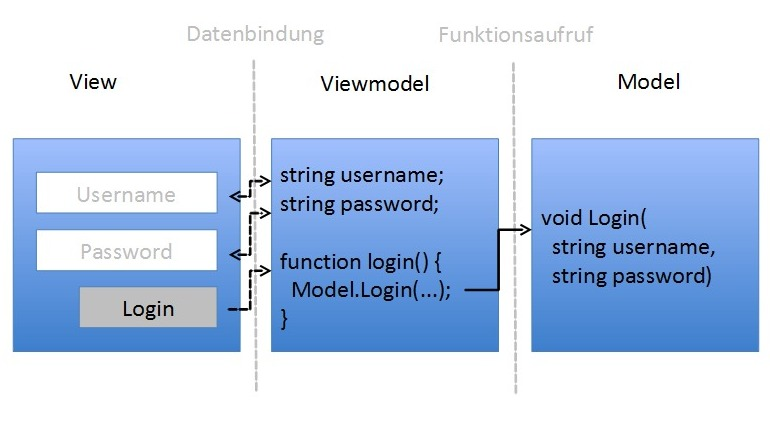
\includegraphics[width=0.7\textwidth]{./img/tech-ana/mvvm.jpeg}
	\caption{MVVM pattern, source \autocite{heise_knockout}}
	\label{fig:mvvm}
\end{figure}

Knockout also provides a more convenient way to define the properties of a ViewModel, the mapping plugin.
The mapping plugin converts any property of any JSON object to a Knockout observable in order to act as ViewModel.
Listing (\ref{ko_mapping}) shows the previously introduced name example with the mapping plugin.

\begin{lstlisting}[label=ko_mapping,caption=the mapping plugin]
var person = {
	firstName : 'Daniel';
	lastName : 'Meiers';
	fullname : function({
			return firstname +lastName;
		});
var viewModel = ko.mapping.fromJS(person);
\end{lstlisting}

Knockout JS does not support attaching a server side backend or REST API.
Furthermore, it is not able to route between different pages of your application.
Thus these parts of the application has to be implemented by the user or an additional frameworks must be used.

\subsubsection{Ember JS}

Ember JS is one of the younger frameworks, mainly created by Yehuda Katz and Tom Dale and introduced in December 2011 \autocite{tech-ana:announcing-ember}.
In this short time Ember JS could make a really impressive progress and has gained a lot of attraction which can be concluded from the number of github stars and watches.
It comprises all necessary parts for building web applications including two way data binding with templates, a routing mechanism and provides a way to connect the application to REST APIs.

Ember is a very stringent and opinionated framework and is built upon concepts such as DRY (dont repeat yourself) and CoC (Convention over Configuration).
Especially the usage of naming conventions allows it to write applications with a minimal amount of code.
The disadvantage of this is that it is more sophisticated to get started with Ember.js because the philosophy and the concepts of Ember need to be understood first.
The full stack and opinionated approach are the reason why Ember is one of the largest frameworks (56k).

It uses Handlebars as templating engine which is a very popular string based templating engine.
Ember.js also provides a way to connect your application to RESTful WebServices with an additional project, ember-data.
As well as Ember itself ember-data highly makes use of the Convention over Configuration principle which means that ember-data expects the data provided by a REST-Service in a special format.
The Ember team substantiate : "[...]we don't think most web developers should have to write any custom XHR code for loading data.
Strong conventions on the client and strong conventions on the server should allow them to communicate automatically." \autocite{tech-ana:ember-data}.
Besides ember-data it is also possible to use any other server connection implementation.

To build an Ember application it is necessary to create an instance of an Ember.Application object (see listing \ref{em_js}) first.
\begin{lstlisting}[label=em_js, caption=app.js]
var App = Ember.Application.create();
\end{lstlisting}

\begin{lstlisting}[label=em_html,caption=index.html]
<html>
    <head>
        <title></title>
        <meta http-equiv="Content-Type" content="text/html; charset=UTF-8">
    </head>
    <body>

    </body>
    
    <script type="text/x-handlebars">
	<div>
	{{outlet}}
	</div>
    </script>

    <script type="text/x-handlebars" data-template-name="index">
	<div>
		<label>First Name</label> 
		<input {{bindAttr value=firstName}}></input>
	</div>
	<div>
		<label>Last Name</label> 
		<input {{bindAttr value=LastName}}></input>
	</div>
	<p>Hello {{fullName}}</p>
   </script>

    <script src="js/libs/jquery-1.9.1.js"></script>
    <script src="js/libs/handlebars-1.0.0-rc.4.js"></script>
    <script src="js/libs/ember-1.0.0-rc.6.js"></script>
    <script src="js/app.js"></script>
</html>
\end{lstlisting}

Creating the application object defines the namespace of the application.
All other classes, like Routers, Controllers, Views or Models are defined as properties of the application object.
This has the advantage that the JavaScript namespace does not get polluted by application depended objects.
Besides some other initialisation the create() statement automatically creates a default router for the application.
The default router first sets up the ApplicationRoute with the ApplicationTemplate, a pre-defined and special route only for application startup.
The ApplicationTemplate is defined in listing \ref{em_html} in line 10.
By convention Ember treats this as ApplicationTemplate because the id attribute of the script tag is missing.

The ApplicationTemplate is the right place for static content like headers, footers or menu bars, in fact it gets always rendered first.
The \{\{outlet\}\} tag tells ember where to fill in dynamic content that depends on the currently loaded route.
After this initialization the Ember router starts the routing process and routes to the current route.
This is normally the plain basic url.
This path is connected per convention to Embers IndexRoute so that the Router takes all steps to initialize the IndexRoute.
One important note to mention here is that the templates are standard handlebars templates.

As outlined before, a very central concept of Ember is routing.
Every Ember application needs a Router because the Router translates a URL into a series of templates and is responsible for loading these templates as well as respective model data and sets up other application state.
Listing \ref{lst:em_router} demonstrates a Router definition with two different routes.

\begin{lstlisting}[label=lst:em_router,caption=Router Defintion in Ember]
App.Router.map(function() {
  this.route("about");
  this.route("favorites");
});
\end{lstlisting}

Embers routing mechanism is a good example how the CoC apporach is used to avoid boilerplate code. As listing \ref{lst:em_router} depicts only the routes itself are defined but no programming logic that defines how to set up the routes. 
This is because a naming convention is used to map the current url to the route name and from the route name to the controller and the template to display.
The table in figure \ref{fig:ember_routes} demonstrates the naming convention.

\begin{figure}
	\centering	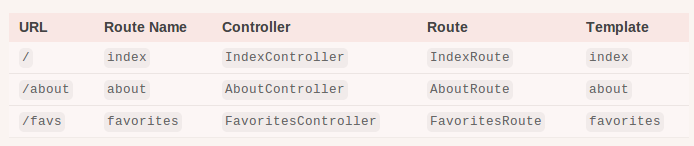
\includegraphics[width=1.0\textwidth]{./img/tech-ana/ember_routes_conventions.png}
	\caption{Ember Conventions for Routes, source \autocite{tech-ana:em-routes-coc}}
	\label{fig:ember_routes}
\end{figure}

Starting the code snippets \ref{em_js} - \ref{lst:em_router} would result in a page showing empty input fields for both properties because the templates that are involved are not backed with a model that contains data for the templates to display.

Every template is backed by a model and the route defines what model should be used by the template.
As depicted in table \ref{fig:ember_routes} ember will look for an App.IndexRoute by convention. So this is the right place to point to the model.

\begin{lstlisting}[label=em_controller,caption=app.js]
var App = Ember.Application.create();
App.Person = Ember.Object.extend({
	firstName: null,
	lastName : null,
    fullName: function() {
        return this.get('firstName') + " " + this.get('lastName');
    }.property('firstName','lastName')
});

var myself = App.Person.create({
    firstName: "Daniel",
    lastName: "Meiers",
});

App.IndexController = Ember.ObjectController.extend({});

App.IndexRoute = Ember.Route.extend({
    model: function() {
        return myself;
    }
});
\end{lstlisting}

In listing \ref{em_controller} a model class called Person is defined first, which has the same properties as in the Knockout example.
In order to do this a special ember class is extended in order to bind to these properties int the templates.
After that an instance of this class is created and the needed properties are set.
In line 15 the controller which should be used for the IndexRoute is declared.
In Ember a controller is the component that manages the UI logic and the application state.
It is comparable to ViewModel object of Knockout.
As mentioned earlier each template is backed by a model.
To be more precise templates retrieve their properties from the controller which decorates the model and provides proxy attributes to avoid for an easier access in the templates. Figure \ref{fig:ember_coupling} visualises how templates, controllers and models are related to each other.
The last step in the IndexRoute object is to point to the model instance.

\begin{figure}
	\centering	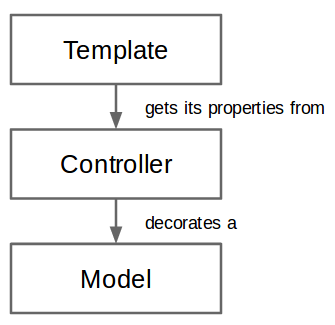
\includegraphics[width=0.45\textwidth]{./img/tech-ana/ember_controller_coupling.png}
	\caption{Ember model coupling, source \autocite{tech-ana:em-coupling}}
	\label{fig:ember_coupling}
\end{figure} 
 
By default it is not necessary to define a controller for the IndexRoute but by convention Ember assumes that the IndexController manages a list of model objects and therefore expects an array for the model property.
Another way to achieve the same thing is demonstrated in listing \ref{em_2}.
A special Ember Array is defined and the created Person instance is added to it. Finally the IndexRoute must point to the array instead.
Since the model is now an array the template needs to be adopted to iterate over all existing array members (see listing \ref{em_array_template}).

\begin{lstlisting}[label=em_2,caption=app.js]
var persons = Ember.A();
persons.pushObject(myself);

App.IndexRoute = Ember.Route.extend({
    model: function() {
        return myself;
    }
});

\end{lstlisting}     

\begin{lstlisting}[label=em_array_template,caption=index.html]
<script type="text/x-handlebars" data-template-name="index">
	{{#each}}
		<div>
			<label>First Name</label> 
			<input {{bindAttr value=firstName}}></input>
		</div>
		<div>
			<label>Last Name</label> 
			<input {{bindAttr value=LastName}}></input>
		</div>
		<p>{{fullName}}</p>
	{{/each}}
</script>
\end{lstlisting}

If that application is started the input fields are properly bound to the model properties.
But if the first name or last name in the input field is changed, these changes are not reflected to the p-element at the bottom of the page.
This is because Ember does not know how to react on events that are fired on user interaction.
To react on user events and enable a two way data binding an Ember View needs to be used instead. Ember Views \enquote{[...] are responsible for responding to user events, like clicks, drags, and scrolls, as well as updating the contents of the DOM when the data underlying the view changes.} \autocite{tech-ana:em-views}.
Luckily, Ember has a small set of built in views which are Ember.Checkbox, Ember.TextField, Ember.Select and Ember.Textarea.
If necessary it is also possible to create custom views.
Therefore the only thing that needs to be changed is to replace the input element with an Ember.TextField view as demonstrated in listing \ref{em_view}

\begin{lstlisting}[label=em_view,caption=Ember Views]
	{{view Ember.TextField valueBinding="firstName"}}
\end{lstlisting}

As mentioned earlier Ember also provides a way to automatically connect Ember Models to an REST API. However this module does not come up with further concepts that are relevant to understand the Ember framework itself.

\subsubsection{Angular JS}  

AngularJS is developed by Google and has become one of the more popular Frameworks.
AngularJS follows a slightly different apporach compared to the other frameworks.
This approach is best described by the Angular developers itself: \enquote{Angular is what HTML would have been had it been designed for applications} \autocite{tech-ana:ng-intro}.
One aspect that shows the difference of Angular are the so called directives, which are a key concept of AngularJS.
Directives allow the user to extend the native HTML with new and application dependent functionality.
This is done by introducing new HTML tags or attributes, as well as some JavaScript code that defines the behaviour and a way how to convert the new introduced tag and the current model state into plain old HTML. Using directives extensively, HTML can be turned into a declarative domain specific language (DSL).

%The second aspect Angular differs from the other frameworks is the templating system.
%(angular docu says that the template system is DOM based ?)   

Furthermore AngularJS also provides two way data binding, filters, routing and dependency injection.
All these components and features make it easy to write Single Page Web Applications without writing any sort of boilerplate code, assuming the architecture and concepts of Angular JS are well known.

%(this is one the disadvantages, takes much time to get familiar with angular)  

%- is the one with the most community activity (github forks, stars, watches) 

Listing \ref{angularBasic} shows the very simple implementation of the same app used before.
The special here is that it is not necessary to write one line of JavaScript code to get things work.
Unfortunately this example isn't very intuitive and it seems that there happens a lot of magic behind the scenes.
In the following sections the details of the example and the important concepts of AngularJS are explained.

\begin{lstlisting}[label=angularBasic,caption=First Angular application]
<html ng-app>
    <head>
        <meta charset="utf-8">
        <title>My AngularJS App</title>
    </head>
    <body ng-init="firstName='Daniel'; lastName='Meiers';">
        <div>
            <label>First Name</label> 
            <input ng-model="firstName"></input>
        </div>
        <div>
            <label>Last Name</label> 
            <input ng-Model="lastName"></input>
        </div>
        <p>Hello {{firstName}} {{lastName}}</p>
        <script src="lib/angular/angular.js"></script>
        <script src="js/app.js"></script>
    </body>
</html>
\end{lstlisting}

The first thing to mention here is the ng-app directive.
This directive defines the application root and Angular automatically looks for this directive during page load.
If found, it starts bootstrapping the angular application which basically means three things:
\begin{itemize}
	\item load the module associated with the directive.
	\item create the application injector
	\item compile the DOM treating the ng-app directive as the root of the compilation.
\end{itemize}

Using this special directive as the root of the Angular related content has the advantage that only a part of the total application can be handled by Angular and the context of the Angular application can be restricted to a part of the DOM.
This makes it much easier to migrate Angular into existing projects or to combine Angular with other frameworks.

In Angular the application consists of one or more so called Modules.
Modules \enquote{[...] declaratively specify how an application should be bootstrapped} \autocite{tech-ana:ng-module}.
This is necessary since Angular applications does not have a main method which can make the instantiation process.
The Module that should be loaded can be referenced in the ng-app directive.\\[5mm]

\begin{lstlisting}[label=ngModule,caption=ng-app declaration with module]
<html ng-app="myApp">
....
<script type="text">
	var myAppModule = angular.module('myApp', []);
</script>
....
\end{lstlisting}

The first parameter of the module creation (line 4 of listing \ref{ngModule}) defines the name of the module that must be used for referencing it in the ng-app directive.
The second parameter can be used to define other modules as dependency for this module.
These dependent modules are created first and then injected into the module per Dependency Injection.
Among others,the most notably advantage of this approach is, that the separation in modules simplifies unit testing, since not all modules must be loaded for unit testing and additional modules can be loaded, that, can provide some mock up functionality for testing.
This helps writing end-to-end test for the application and allows easily testing the GUI behaviour with unit tests. 

In our simple application (see listing \ref{angularBasic}) we have not defined a module that should be loaded. 
Therefore angular loads a default module.
This default module initializes the application wide Injector which is responsible for the Dependency Injection.
The last step of bootstrapping comprises the re-compilation of the DOM.
Each found Directive or binding expression is evaluated and translated into plain HTML.

The next directive we used in \ref{angularBasic} is the ng-init directive.
this directive allows to do initialisation tasks before the app starts running.
The ng-init directive automatically creates a new property on the corresponding scope object and sets the respective initial values for it, that are declared in the expression. A more detailed explanation of the scope concept is given later on, but in short, the scope in Angular can be compared with the ViewModel object in Knockout.
The ng-model directive binds those properties to the element it is defined in, which automatically enables a two-way data binding between the model properties and the view.
The automatic creation of model properties, is an important difference compared to Knockout and Ember, where this needs to be done manually.  
Before explaining this feature in more detail it is necessary to have a closer look on Angualars scope concept which also requires to understand the meaning of Models, Views and Controllers in the Angular architecture.

The Scope is an object that refers to the application model and provides necessary context for Expressions and directives.
An Angular expressions are a JavaScript-like code snippets that are usually places in data-bindings and can be used for accessing model properties and some basic calculations.
Scopes can watch Angular expressions and propagate events.
These features are used also internally to implement the two way data binding.
Scopes are the "glue between application controller and the view" \autocite{tech-ana:ng-scope} and are comparable to Knockouts ViewModel.
An Angular application always consists of exactly one RootScope and multiple ChildScopes.
They are hierarchical nested and resemble the DOM structure as figure \ref{fig:angular_scopes} depicts.
Similar to the model declaration, this can also happen implicit by directives like the ng-repeat directive in figure \ref{fig:angular_scopes}.
ChildScopes prototypically inherit from their parent scope.
Hence, if an binding expression like {{firstName}} is evaluated, Angular first checks if the Scope object related to that element contains this property.
If not it checks all parent scopes until the property is found or the RootScope is reached.

\begin{figure}
	\centering	
	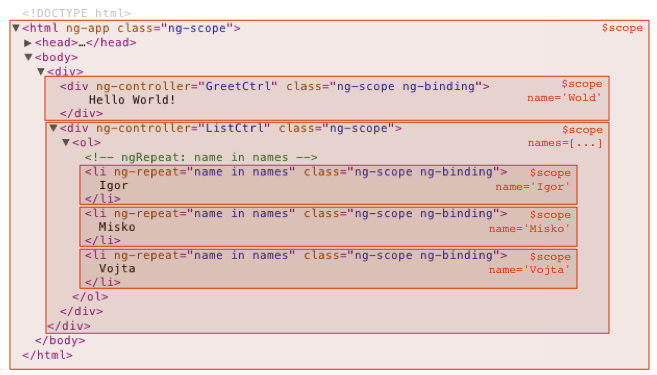
\includegraphics[width=0.8\textwidth]{./img/tech-ana/angular_scopes.png}
	\caption{Hirarchie of Angular scopes, source \autocite{tech-ana:ng-scope}}
	\label{fig:angular_scopes}
\end{figure} 

In Angular a Model can be any JavaScript object including Arrays and primitives.
The only condition is that it must be referenced by a Scope object.
The name of the scope property is also the model identifier that can be used for accessing the value in expressions.
The creation of models can be done explicit or implicit.
In listing \ref{angularBasic} the model is created implicit with the ng-model directive.
To create a model explicit it is necessary to add new properties to the scope in the corresponding Controller.

As already mentioned, Controllers are also a way to create models in Angular and adding them to the Scope.
Controllers are JavaScript functions that are used to augment the Angular scope and are normally used to set up initial state of the Scope or to add application behaviour to it.
Listing \ref{angularController} depicts the needed changes.

\begin{lstlisting}[label=angularController,caption=Angular Controller]
<html>
....
<body ng-controller="HelloController">
....
<script type="text">
	function HelloController($scope){
	    $scope.lastName = "Meiers";
	    $scope.firstName = "Daniel";
	};
</script>
...
\end{lstlisting}

There are two ways how Controllers are associated with Scope objects.
The first one is to use the ng-controller directive as in the example above.
The second one is to use Angulars Routing mechanism.
Another important thing to mention here is that the Scope object is provided by Angulars DI (Dependenci Injection) system.
  

The last component to cover all elements of the MVC pattern is the View.
In Angular the view consists of the loaded and rendered DOM after Angular has transformed Angular specific directives and expressions into normal HTML.
Figure \ref{fig:angular_views} are giving a good overview over this process.
  
\begin{figure}
	\centering	
	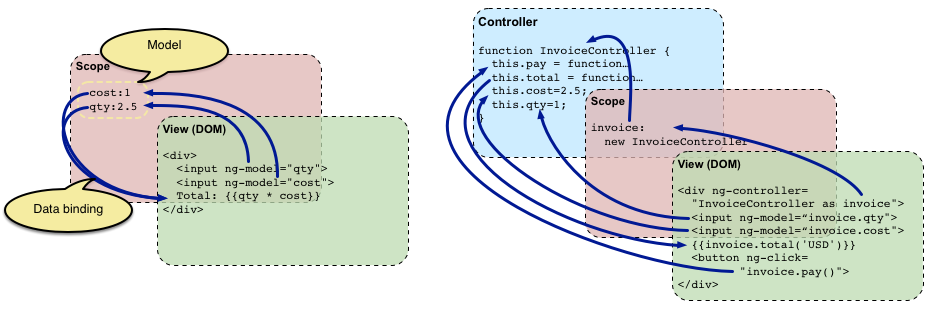
\includegraphics[width=1.0\textwidth]{./img/tech-ana/angular_view.png}
	\caption{Functionality of Angular Views, source \autocite{tech-ana:ng-concepts}}
	\label{fig:angular_views}
\end{figure} 

There are a few more concepts in Angular that helps and simplifies SPA development with Angular.
A really useful feature that makes Angular outstanding are Filters.
Filters are a way to format data that should be displayed to the user.
For example, if we want to print the fullName property of our basic example in uppercase letters we just need to use the Uppercase filter provided by Angular (see listing \ref{angular_filters}).
Angular already provides a basic set of very useful Filters among them Filters for ordering or filtering lists of data but it is also possible to create custom ones.
Filters are used in Angular expressions with an pipe like syntax.

\begin{lstlisting}[label=angular_filters,caption=Angular Filters]
 {{ fullName | uppercase}}
\end{lstlisting}

The last concept are Services.
Services in Angular apps are substitutable objects that are wired together using dependency injection. Angular Services are implemented as singletons and are used to carry out specific tasks common to web apps and reusable business logic independent of views. Angular provides an impressive set of services such as the \$http service that provides low level access to the browser's XMLHttpRequest object and can be used to make AJAX requests.

The routing mechanism is also implemented as service. This has the advantage that it can be easily injected by dependency injection in every module that wants to use the routing mechanism. The oruting service tries to map the path of the current location to an existing route definition. Listing \ref{lst:ng-routes} demonstrates that a route definition basically consists of the template that should be loaded and the controller function the route is related with. The url the route is defined for can also contain dynamic parts, for example the bookId field, that indicates the controller which book object shall be displayed.

\begin{lstlisting}[label=lst:ng-routes,caption=Route definition in AngularJS]
var mod = angular.module('ngViewExample', ['ngRoute'])
 
mod.config(function($routeProvider, $locationProvider) {
  $routeProvider.when('/Book/:bookId', {
    templateUrl: 'book.html',
    controller: BookCntl
    }
  });
  $routeProvider.when('/Book/:bookId/ch/:chapterId', {
    templateUrl: 'chapter.html',
    controller: ChapterCntl
  });
  
  function BookCntl($scope, $routeParams) {
	....
  }
});
\end{lstlisting}

\subsection{Discussion} \label{chap:fw-discussion}


After giving a first introduction into the concepts of Knockout.js, Ember.js and AngularJS, it is necessary to discuss the pros and cons of the different frameworks.

Knockout JS very reduced feature set can be both, a blessing and a curse and it depends on the needs to decide what of these two things prevails.
Knockout JS is a very easy to learn library hence there are only a few concepts to learn.
Another benefit of Knockout JS is, that it has a widely spreaded browser support also for older browser versions.
This benefit is not that much relevant since the applications to develop should be rendered in the JavaFX WebKit component.
Knockout is a very flexible framework hence there are  no regulations for defining the structure and architecture of your application.
The missing features of Knockout JS like routing can be compensated with one of the other dozen available third party libraries for this feature.
Unfortunately, without these additional dependencies Knockout JS is rather less suited for building more complex web applications in fact that it forces you to implement too many things manually.
And the additional amount of dependencies could lead to inconsistency problems, increases the error likelihood and the maintenance efforts and make the development even harder (cf \autocite{heise_knockout}).  

Ember however, covers all needed aspects of developing SPA's.
It is possible to write applications with a minimal amount of code, and its concept scale very well, which means it is very easy to write simple applications with Ember that reduces the amount of boilerplate code to a minimum, but the underlying concepts cover also the possibility to create large and complex Single Page Web Applications. With the concept of Ember Components, it is possible to develop reusable components that are furthermore planned to support the upcoming web components standard. 
The only disadvantage is, that Ember is a very strict and opinionated framework.
This is especially true for ember-data which relies heavily on naming conventions to properly work.
Although using approaches like Convention over Configuration is not a principal disadvantage, the question is, if the very stringent corset of Ember will limit further developments or produces a lot of efforts to work around the built in framework concepts.
Ember-data is a good example for that.
Ember-data makes highly use of naming conventions and makes assumptions on the structure of the REST API of the backend. Hence the RESTful API is already defined, it is very likely that the assumptions of ember-data will not correlate with cids REST API, which means that the concepts of the framework need to be work around.
It can not be ruled that similar problems could also arise in other parts of the framework, for example the routing mechanism. 

At this point, the concepts of dependency injection, and services, makes Angular much more flexible.
Similar to Ember, Angular is also capable of building all kind of applications, from the simple to the complex one.
From special interest is the very central concept of directives, which can be used to easily develop reusable components. The angular developers claim, that they will support compatibility of directives to the upcoming web component standard.
The large number of concepts makes it a bit harder to get familiar with Angular, but if the concepts are clear, it is very intuitive to build applications with Angular.
Outstanding points of Angular are besides directives, the usage of Dependency Injection, which allows to easily reuse developed Filters, Services and Modules. Additionally the dependency injection increases the testability of the applications and gives the possibility to easily write end to end unit tests. 

Regarding the performance of Angular and Ember there are some important notes to mention. As outlined in chapter \ref{chap:web_dev} Angular and Ember follow two very different approaches for achieving data binding. In Ember it is necessary to use special objects for the model. Those objects makes it possible to notify about changes. In Angular it is possible to bind to arbitrary JavaScript objects. It uses dirty-checking to test if any of the binded objects has changed.
The two approaches have some fundamental consequences.
The first and most obvious one is that using dirty checking means that it is possible to bind directly to native JavaScript objects.
This makes the binding expressions slightly more intuitive since no get or set functions are needed to access the properties.
Furthermore it is not necessary to wrap object into  framework depended observable object.
On the other side, the general approach to periodically check the bound JavaScript objects for changes seems to be time consuming and slow.
Although this is conceptually true, this statement needs to be qualified in the practical context.
A good discussion regarding this issue can be found at \autocite{tech-ana:ng-binding}.
The main arguments mentioned there are, that dirty checking is only problematic for a large number of objects and that the human eye can not recognize changes faster than a 50 ms.
There need to be a large amount of objects to check before the 50 ms are exceeded and the user can recognize a sluggish UI.

In addition, also Ember has performance bottlenecks. 
In \autocite{binding_comparison}, Marius Grundersen reveals and discusses the weaknesses of Ember and Angular and demonstrates them with a simple example. 
Figure \ref{fig:demo_app} demonstrates the structure of the demo application. It mainly conists of a input fiels which binds the inserted text to a label above. 
Furthermore, multiple thousands items are added by clicking a button. 

\begin{figure}
	\centering	
	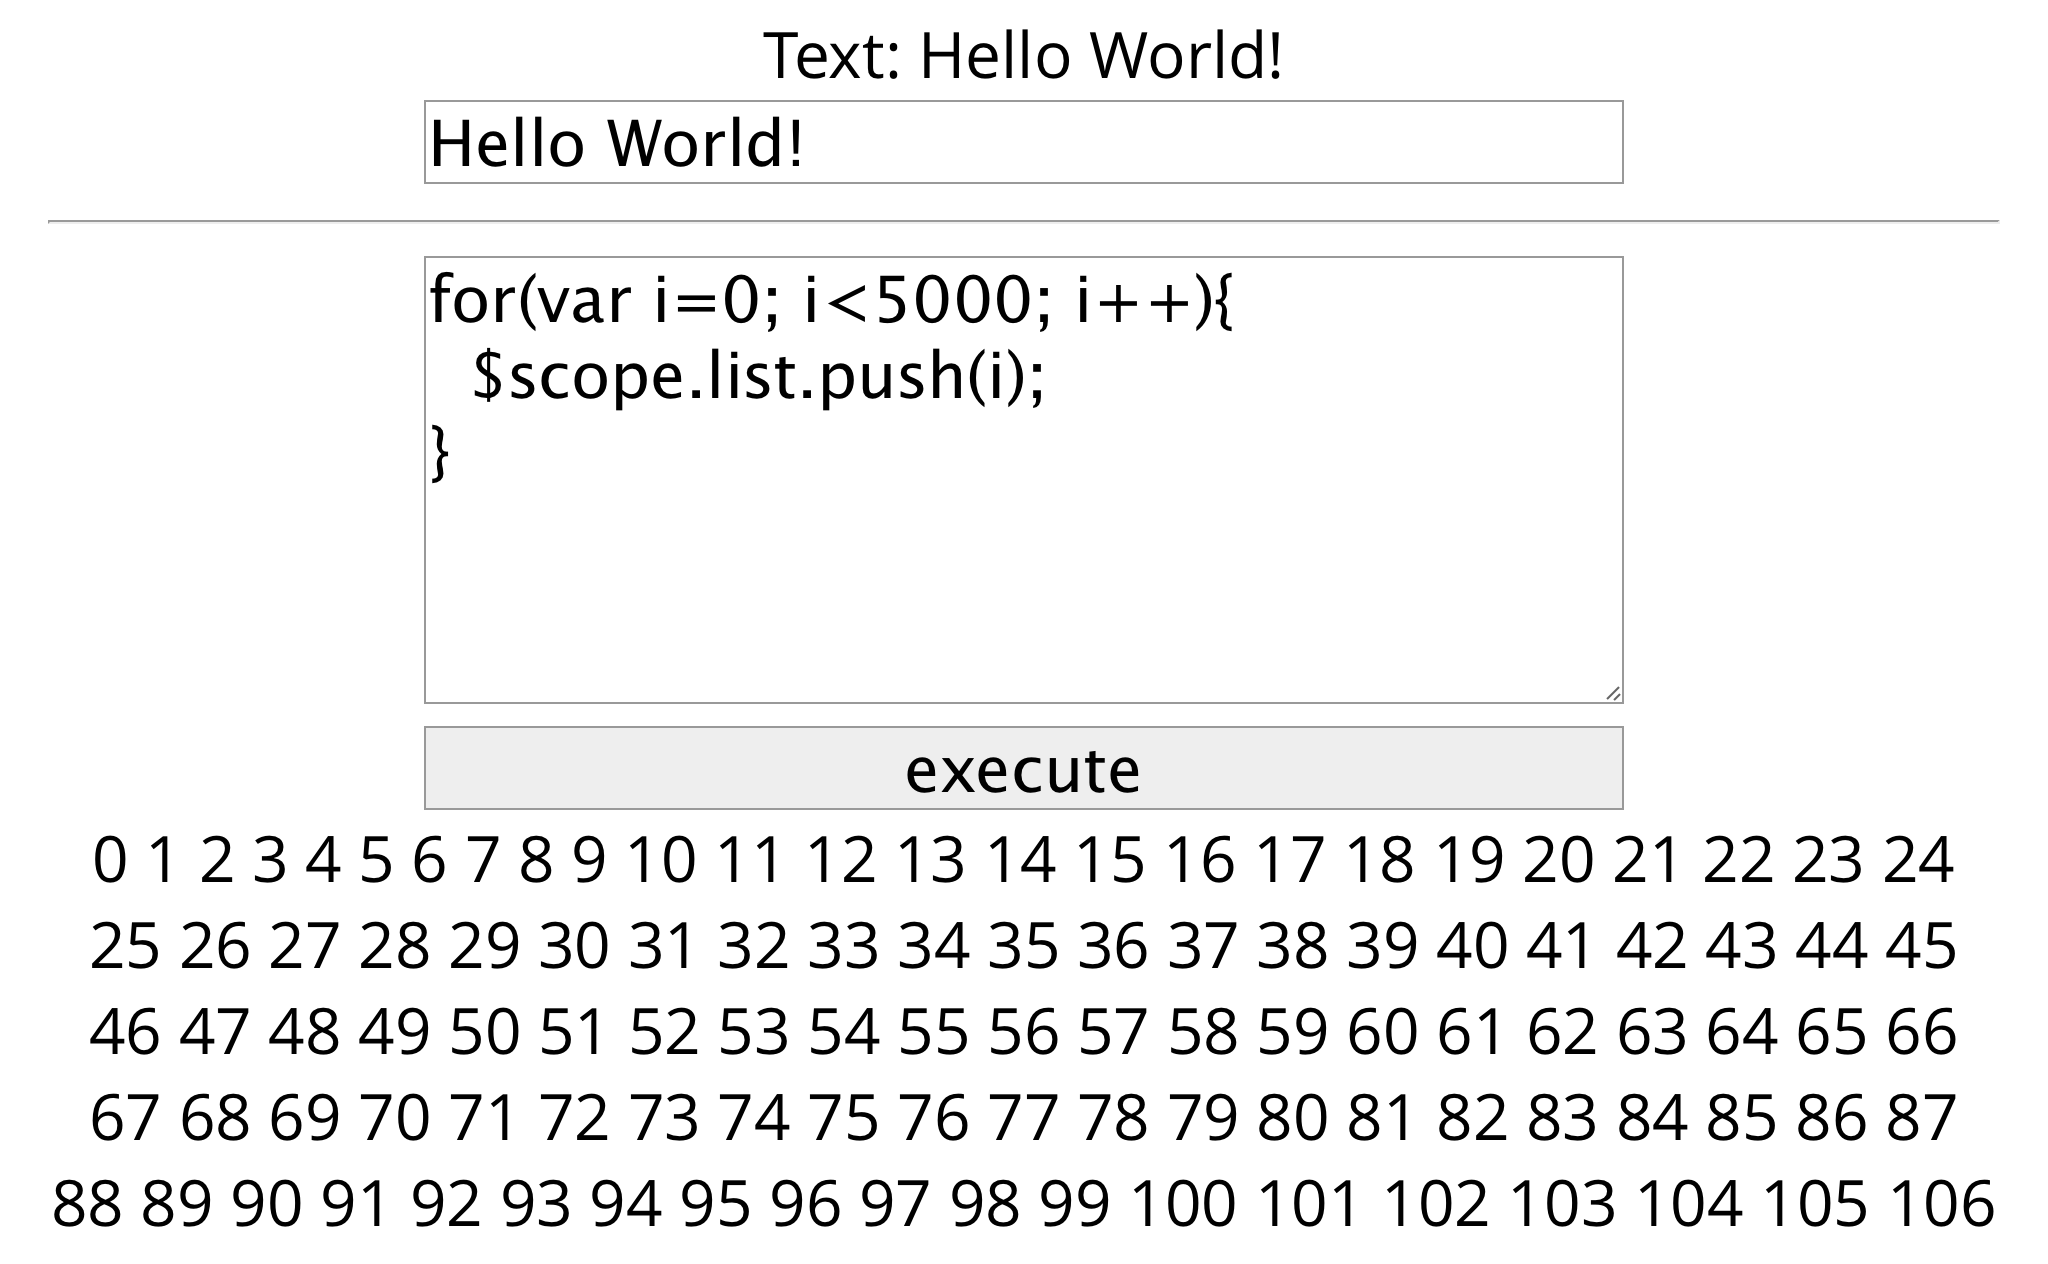
\includegraphics[width=0.8\textwidth]{./img/tech-ana/performance_demo_app.png}
	\caption{Demo Application, source \autocite{binding_comparison}}
	\label{fig:demo_app}
\end{figure} 

Executing this example in Ember reveals that it takes a considerably time until all list items are rendered.
Figure \ref{fig:performance_demo_app} demonstrates the time that is needed for this example. 
Important to note is, that Angular is much faster in that case despite the dirty checking approach. 
The reason for this is, that in Ember it is necessary to set up the notification mechanism for the 5000 objects.
To be fair, the disadvantage of dirty checking first appears when typing in the text field after the list is rendered. 
In this case Angular needs to check all 5000 items although only 1 has changed. 
This makes typing a bit sluggish. 
This example impressively demonstrates that both approaches can have bottleneck effects and it depends on the developer to regard the performance when developing the application. 
A simple solution to avoid the bottleneck affect in Angular is two use multiple scopes.

\begin{figure}
	\centering	
	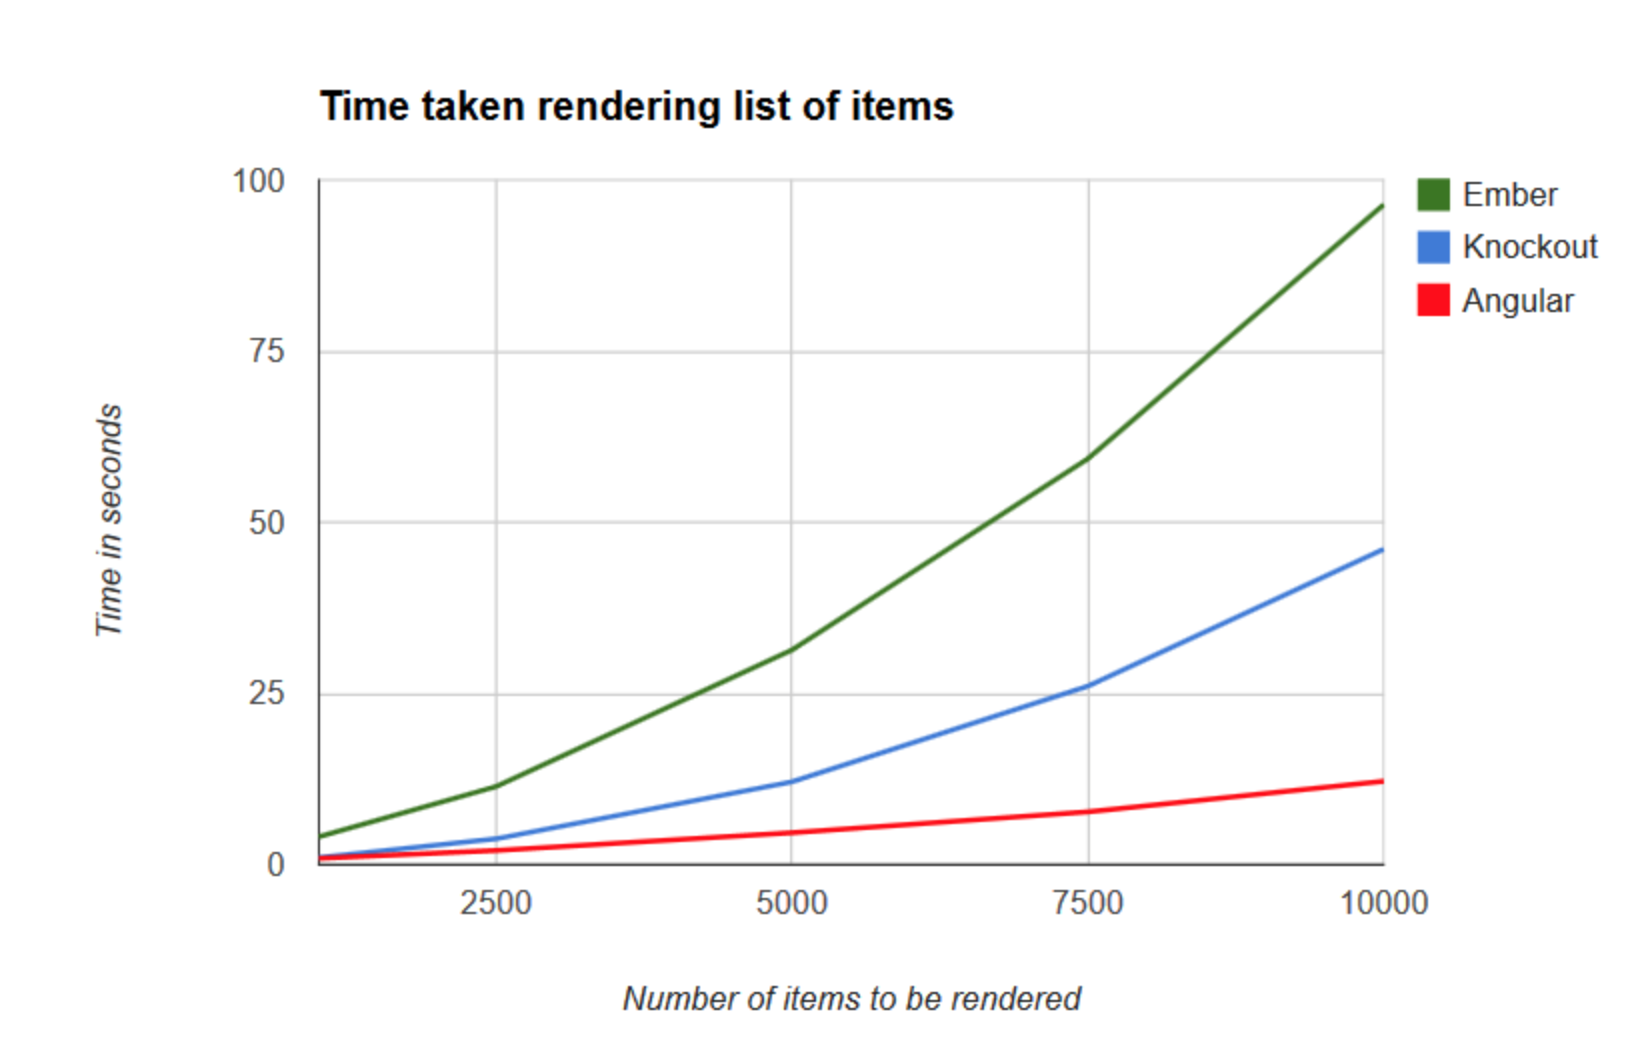
\includegraphics[width=0.8\textwidth]{./img/tech-ana/performance_comp.png}
	\caption{Performance Comparison of Demo Application, source \autocite{binding_comparison}}
	\label{fig:performance_demo_app}
\end{figure} 

Another important part that is also listed in the requirements in chapter \ref{chap:requirements} is the documentation, the community support and the existence of test tools. 
But also here the difference between Ember and Angular are more from a marginal nature. 
The documentations are both very extensive and from a good quality. 
There a many examples that allow to easily use the frameworks. 
Furthermore the documentaion of  Ember as well the Angular documentation both provide tutorial ans How-To articles. 
However, from a subjective point of view, it appears the the Angular documention has a slight advantage, which may be due to the fact that Ember is the much younger framework. 
The maturity of Angular can also be the reason for the larger community and popularity of the framework. 
But again, for bot frameworks it is easy to find information or get help. 

Regarding the support of test and debugging tools it seems that Angular has a slight advantage hence it has a very good built in testability and also provides a debugging tool Batarang. Batarang helps to examine the scope structure the application and helps monitoring and optimzing the performance. Unfortunately Batarang is only available as Google Chrome extension and cannot be used in the JavaFX WebView.

Summing up, Knockout.js can not be used, hence it has a reduced feature set and does not offer a routing mechanism or reusable components. Embers very stringent and opinionated approach bears the danger that the framework can limit future developments and complicated and sophisticated workarounds are necessary. Hence AngularJS has none of the above mentioned disadvantages, it is clear that AngularJS is the most promising candidate and shall be used for the further considerations. Table \ref{tbl:js-fw-comp} gives an overview over the different features of each framework and allows a more accessible comparison of them. The disqualifying factors are emphasized with with a coloured background. Up to know the conception of the new required feature is outlined, and the most suiting candidate regarding the browser API as well as a JavaScript MVC Framework is evaluated. Now, that all prerequisites are fulfilled it is possible to start with the implementation.



\label{tbl:js-fw-comp}
%\todo{ emph disqualifying factors}
	\begin{tabular}{|m{2.8cm}|>{\centering\arraybackslash}m{3.5cm}|>{\centering\arraybackslash}m{3.5cm}|>{\centering\arraybackslash}m{3.5cm}|}
	\hline
	\rowcolor{gray}
		& \head{Angular JS	} & \head{Ember JS} & \head{Knockout JS}	  \tabularnewline
		\hline
	2-way data binding	 		
		& \checkmark
		& \checkmark
		& \checkmark  \\ \hline
	normal and computed properties	
		& \checkmark / change detection
		& \checkmark / \checkmark
		& \checkmark / \checkmark\\ \hline
	Testing				
		& end-to-end tests, build in tools for unit tests,debugging extension for chrome 
		& extra packages ember-testing,qUnit 
		&  unit tests \\ \hline
	Routing				
		& \checkmark 
		& \checkmark	
		& \cellcolor{LightRed} -		\\ \hline
	Multiple and Composite Views	
		& \checkmark / \checkmark
		& \checkmark / \checkmark 
		& \cellcolor{LightRed} -		\\ \hline
	Backend connection		
		& optional (ajax wrapper)	
		& optional (ember-data)	
		& -	\\ \hline
	%Dependency injection
	%	& \checkmark
	%	& -
	%	& -\\ \hline
	%Templating system
	%	& Dom based 
	%	& String based (handlebars)
	%	& Dom based\\ \hline
	Documentation
		& very good
		& good
		& good\\ \hline
	API stability / maturity
		& since 2009, stable
		& since 2011, 
		&since 2010, very stable\\ \hline
	community (github watch/star/fork
		& 1450/13061/3147
		& 672/7752/1568
		& 349/4074/657\\ \hline
	Perfomance
		& slowest when the model is complex
		& slowest when rendering large lists
		& slowest when pushing many items\\ \hline
	Flexibile vs opinonated
		& flexible
		& \cellcolor{LightRed} stringent \& opinionated
		& flexible\\ \hline
	%size
	%	& 80kb
	%	& 56kb + JQuery + Handlebars
	%	& 15kb\\ \hline	
	%FrameWork / Library
	%	& Something in between
	%	& Framework
	%	& Library\\ \hline
	Integration of UI Elements
		& \checkmark use directives
		& \checkmark use Ember views
		& \checkmark use custom bindings \\ \hline
	License
		& MIT License
		& MIT License
		& MIT License\\ \hline
	\end{tabular}

